\documentclass{./../div_teaching_slides}

\begin{document}
\title{ECON 340 \\ Economic Research Methods}
\author{Div Bhagia}
\date{Lecture 20 \\ Quadratic and Log functional forms}

%%%%%%%%%%%% 
\begin{frame}[noframenumbering, plain]
\maketitle
\end{frame}

%%%%%%%%%%%%%%%%%%%%
\begin{frame}{Remember Calculus?}
For a function $$ y = f(x) $$
The derivative denoted by:
 $$\frac{dy}{dx} \quad or \quad f'(x) $$ captures how the value of the function changes due to a small change in $x$.
\end{frame}

%%%%%%%%%%%%%%%%%%%%
\begin{frame}{Rules of Differentiation}
\begin{witemize}
\item $\displaystyle y=a  \rightarrow  \frac{dy}{dx}=0$
\item $\displaystyle y=ax \rightarrow \frac{dy}{dx}=a$
\item $\displaystyle y=ax^b \rightarrow  \frac{dy}{dx}=abx^{b-1}$
\item $\displaystyle y=f(x) + g(x) \rightarrow  \frac{dy}{dx}=f'(x) + g'(x)$ \\~\\
\end{witemize}
\textit{Examples}: $ y = 10,  \quad  y = 5x,  \quad y = 8x^3,  \quad y = 3x^2 + 4 $
\end{frame}


%%%%%%%%%%%%%%%%%%%%
\begin{frame}{Rules of Differentiation}
\begin{witemize}
\item Derivative of a log function:
$$ y=log(x) \quad \rightarrow \quad \frac{dy}{dx}=\dfrac{1}{x}$$
\item Chain rule:
$$z=f(y),\ y=g(x) \quad \rightarrow \quad \frac{d z}{d x}=\dfrac{d z}{d y} \cdot \frac{d y}{d x}$$
\end{witemize}
\textit{Examples}: $ y = 2 + 3 \cdot log(x),\  y = log(z) \ \& \ z = x^2,\    y = log(x^2), \ y = log(f(x)) $
\end{frame}

%%%%%%%%%%%%
\begin{frame}{Fitting a Line}
Linear relationship (with some error):
$$ Y = \beta_0 + \beta_1 X + u  $$

Taking the conditional expectation:
$$ E(Y | X) =  \beta_0 + \beta_1 X + E(u | X)  $$

With $E(u | X)=0$, 
$$ E(Y | X) =  \beta_0 + \beta_1 X   $$

OLS fits a linear line between average $Y$ at each $X$ and $X$. 
\end{frame}

%%%%%%%%%%%%
\begin{frame}{ACS Data: Wages and Age}
\centering Is the relationship really linear? \\ \vspace{1em}
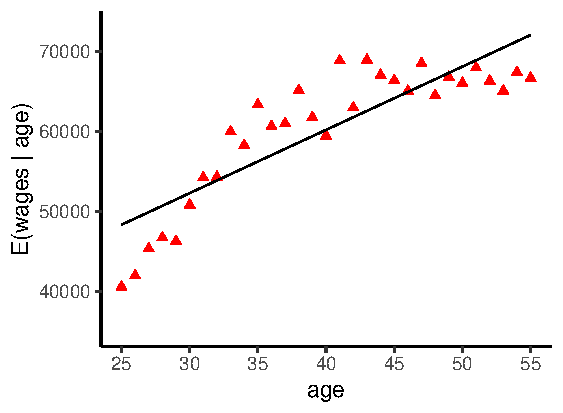
\includegraphics{./../../output/scatter_age_wage_lfit.pdf}
\end{frame}

%%%%%%%%%%%%
\begin{frame}{ACS Data: Wages and Age}
\centering Does this model have a better $R^2$? \\ \vspace{1em}
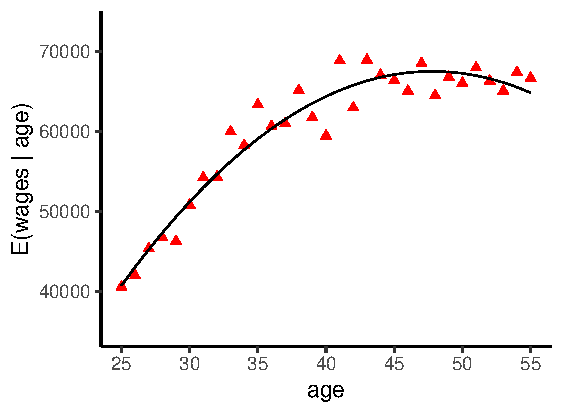
\includegraphics{./../../output/scatter_age_wage_qfit.pdf}
\end{frame}

%%%%%%%%%%%%
\begin{frame}{Fitting a Line}
Linear relationship:
$$ \hat{Y} = \hat{\beta}_0 + \hat{\beta}_1 X   $$

Take the derivative:
$$ \frac{d \hat{Y}}{dX} = \hat{\beta}_1 \rightarrow d \hat{Y} = \hat{\beta}_1 dX  $$ \\~\\

Can think of $d$ as `change in':
One unit change in $X$, associated with $\beta_1$ units change in $Y$. \\~\\
Impact of $X$ on $Y$ constant with $X$. \\~\\
\end{frame}


%%%%%%%%%%%%
\begin{frame}{Fitting a Curve}
Quadratic relationship:
$$ \hat{Y} = \hat{\beta}_0 + \hat{\beta}_1 X + \hat{\beta}_2 X^2   $$

Take the derivative:
$$ \frac{d \hat{Y}}{dX} = \hat{\beta}_1 + 2 \hat{\beta}_2 X $$ \\~\\

Now the impact of $X$ on $Y$ changes with $X$. \\~\\
Remember: Derivative captures the slope of the tangent line.

\end{frame}

%%%%%%%%%%%%
\begin{frame}{ACS Data: Wages and Age}
\centering \vspace{-2em}
$$ \hat{wage} = -52207 + 4775.64 \cdot age -49.493 \cdot age^2   $$
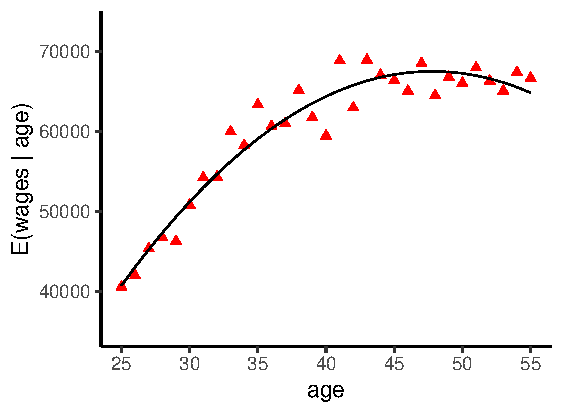
\includegraphics{./../../output/scatter_age_wage_qfit.pdf}
\end{frame}

%%%%%%%%%%%%
\begin{frame}{ACS Data: Wages and Age}
$$ \hat{wage} = -52207 + 4775.64 \cdot age -49.493 \cdot age^2   $$
\vspace{1em}

How does the predicted wage change going from 30 to 31? \\~\\ \vspace{2em}

What about going from 50 to 51?
\end{frame}

%%%%%%%%%%%%
\begin{frame}{Log Functional Forms}
\vspace{-0.75em}
Sometimes we  log transform a variable before fitting a model. Useful if the data is skewed or has outliers.\vspace{-0.25em}
 \begin{columns}[T]
\begin{column}{0.5\textwidth}
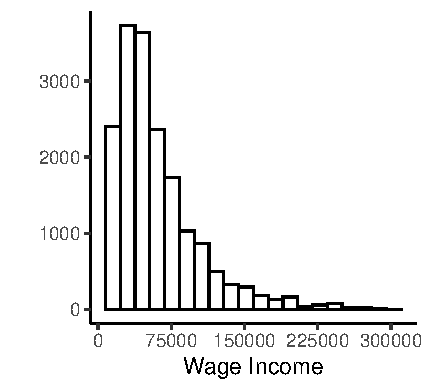
\includegraphics{./../../output/lrm_ff_hist_wages.pdf}
\end{column}	
\begin{column}{0.65\textwidth}
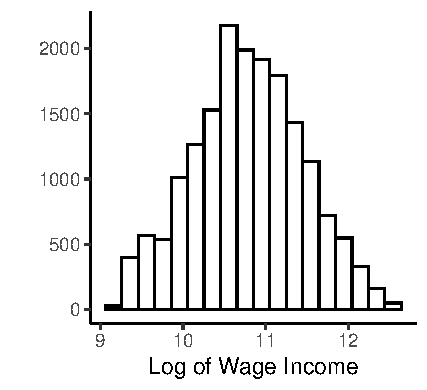
\includegraphics{./../../output/lrm_ff_hist_lwages.pdf}
\end{column}	
\end{columns}
\end{frame}

%%%%%%%%%%%%
\begin{frame}{Log Functional Forms}
\vspace{-0.5em}
\begin{witemize}
  \item Log-transformation leads to interpretation of regression coefficients in \% changes than unit changes which can sometimes be more informative 
  \item Can think of change in log of X as the relative change in X with respect to its original value
  $$ \frac{d}{dX} \log(X) = \frac{1}{X} \rightarrow d \log(X) = \frac{d X}{X} $$
  In which case $100 \times d\log(X)$ represents \% change in $X$
\end{witemize}
\end{frame}

%%%%%%%%%%%%
\begin{frame}{Log Functional Forms: Interpretation}
Three possible models:
$$\text{1. Level-Log:} \quad \hat{Y} = \hat{\beta}_0 +  \hat{\beta}_1 log(X) \hspace{5cm}$$

Differentiating both left and right hand side with respect to $X$:
$$ \frac{d \hat{Y} }{d X} = \hat{\beta}_1 \cdot \frac{1}{X} \quad  \rightarrow  \quad \hat{\beta}_1 = \frac{d \hat{Y} }{d X/X} $$
In which case,
$$ \frac{\hat{\beta}_1}{100} = \frac{\text{unit change in $Y$}}{\text{\% change in $X$}}  $$
\end{frame}

%%%%%%%%%%%%
\begin{frame}{Level-Log Model}
\centering \small \vspace{-0.5em}

% Table created by stargazer v.5.2.3 by Marek Hlavac, Social Policy Institute. E-mail: marek.hlavac at gmail.com
% Date and time: Tue, Apr 18, 2023 - 13:49:03
\begin{tabular}{@{\extracolsep{5pt}}lc} 
\\[-1.8ex]\hline 
\hline \\[-1.8ex] 
\\[-1.8ex] & Wages \\ 
\hline \\[-1.8ex] 
 Intercept & $-$57,224.83$^{***}$ \\ 
  & (5,008.20) \\ 
  & \\ 
 Log Age & 32,052.27$^{***}$ \\ 
  & (1,363.87) \\ 
  & \\ 
\hline \\[-1.8ex] 
Observations & 17,578 \\ 
R$^{2}$ & 0.03 \\ 
\hline 
\hline \\[-1.8ex] 
\textit{Note:}  & \multicolumn{1}{r}{$^{*}$p$<$0.1; $^{**}$p$<$0.05; $^{***}$p$<$0.01} \\ 
\end{tabular} 
 \\ \vspace{1.5em}
\normalsize \textit{1\% increase in age leads to \$320 increase in predicted wages.} 
\end{frame}

%%%%%%%%%%%%
\begin{frame}{Log Functional Forms: Interpretation}
Three possible models:
$$\text{2. Log-Level:} \quad \hat{log}(Y) = \hat{\beta}_0 +  \hat{\beta}_1 X \hspace{5cm}$$

$$\hat{\beta}_1 = \frac{1}{Y}\cdot \frac{dY}{d X} \rightarrow 100 \hat{\beta}_1 = \frac{\text{\% change in $Y$}}{\text{unit change in $X$}}  $$
\end{frame}

%%%%%%%%%%%%
\begin{frame}{Log-Level Model}
\centering \small \vspace{-0.5em}

% Table created by stargazer v.5.2.3 by Marek Hlavac, Social Policy Institute. E-mail: marek.hlavac at gmail.com
% Date and time: Tue, Apr 18, 2023 - 13:49:03
\begin{tabular}{@{\extracolsep{5pt}}lc} 
\\[-1.8ex]\hline 
\hline \\[-1.8ex] 
\\[-1.8ex] & Log Wages \\ 
\hline \\[-1.8ex] 
 Intercept & 10.31$^{***}$ \\ 
  & (0.02) \\ 
  & \\ 
 Age & 0.01$^{***}$ \\ 
  & (0.001) \\ 
  & \\ 
\hline \\[-1.8ex] 
Observations & 17,578 \\ 
R$^{2}$ & 0.03 \\ 
\hline 
\hline \\[-1.8ex] 
\textit{Note:}  & \multicolumn{1}{r}{$^{*}$p$<$0.1; $^{**}$p$<$0.05; $^{***}$p$<$0.01} \\ 
\end{tabular} 
 \\ \vspace{1.5em}
\normalsize \textit{1 year increase in age leads to 1\% increase in predicted wages.} 
\end{frame}

%%%%%%%%%%%%
\begin{frame}{Log Functional Forms: Interpretation}
Three possible models:
$$\text{3. Log-Log:} \quad \log(\hat{Y}) = \hat{\beta}_0 +  \hat{\beta}_1 \log(X) \hspace{5cm}$$

$$\hat{\beta}_1 = \frac{dY/Y}{dX/X} \rightarrow \hat{\beta}_1 = \frac{\text{\% change in $Y$}}{\text{\% change in $X$}}  $$
\end{frame}

%%%%%%%%%%%%
\begin{frame}{Log-Log Model}
\centering \small \vspace{-0.5em}

% Table created by stargazer v.5.2.3 by Marek Hlavac, Social Policy Institute. E-mail: marek.hlavac at gmail.com
% Date and time: Tue, Apr 18, 2023 - 13:49:03
\begin{tabular}{@{\extracolsep{5pt}}lc} 
\\[-1.8ex]\hline 
\hline \\[-1.8ex] 
\\[-1.8ex] & Log Wages \\ 
\hline \\[-1.8ex] 
 Intercept & 8.99$^{***}$ \\ 
  & (0.08) \\ 
  & \\ 
 Log Age & 0.49$^{***}$ \\ 
  & (0.02) \\ 
  & \\ 
\hline \\[-1.8ex] 
Observations & 17,578 \\ 
R$^{2}$ & 0.03 \\ 
\hline 
\hline \\[-1.8ex] 
\textit{Note:}  & \multicolumn{1}{r}{$^{*}$p$<$0.1; $^{**}$p$<$0.05; $^{***}$p$<$0.01} \\ 
\end{tabular} 
 \\ \vspace{1.5em}
\normalsize \textit{1\% increase in age leads to 0.49\% increase in predicted wages.} 
\end{frame}


\begin{frame}{What's next?}
\begin{witemize}
  \item \textbf{No class on Thursday} (11/09) as I am traveling for a conference. Use this time to review the linear regression model and work on Problem Set 4.
  \item Problem Set 4 is due on the following Tuesday (11/14)
  \item Next week: Regression Analysis in R 
\end{witemize}
\end{frame}

\end{document}